\chapter{Experiments}

\section{Experimental setup}

The developed system has been implemented and tested on the Otter USV in the harbor of Trondheim. The testing area contains various obstacles like boats and jetties, and is shown in \figref{fig:testing-arena}. Since the boustrophedon motions CCPP method performed best in the simulations, only that method has been tested experimentally.

\begin{figure}[h!]
    \centering
	\makebox[\linewidth][c]{
	\begin{subfigure}[b]{0.5\textwidth}
		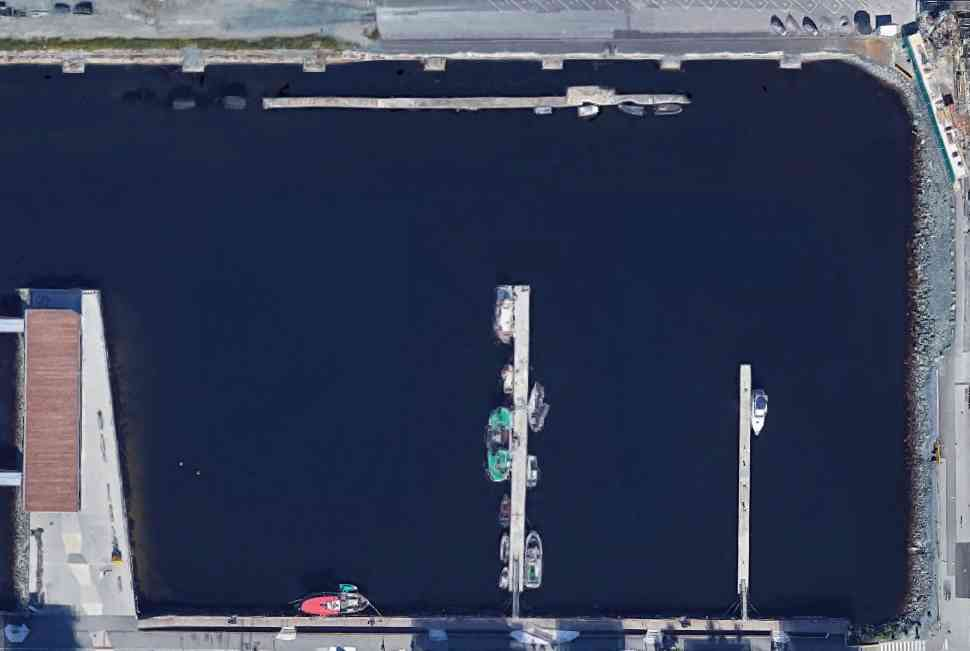
\includegraphics[width=1.0\textwidth]{fig/results/testing-arena2}
		\caption{Top-down view from Google Maps.}
	\end{subfigure}
	\begin{subfigure}[b]{0.5\textwidth}
		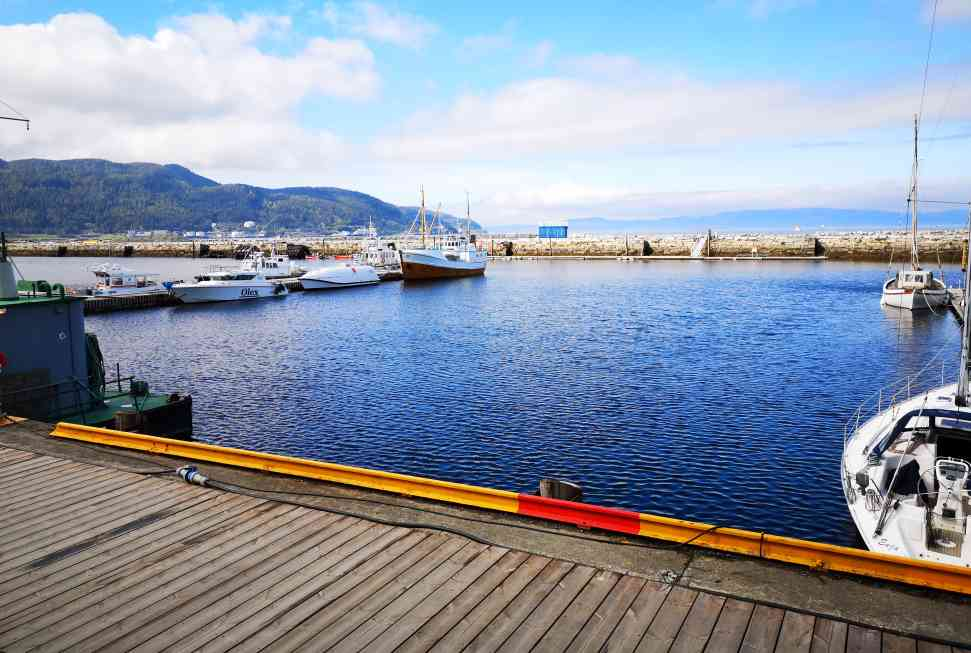
\includegraphics[width=1.0\textwidth]{fig/results/testing-arena-real}
		\caption{Picture on the testing day.}
	\end{subfigure}
	}
	\caption{The testing area used for the Otter USV.}
	\label{fig:testing-arena}
\end{figure}

The Otter USV has not been equipped with a multibeam echosounder during the experiments.  A symmetric constant coverage range is assumed for the MBES instead. Consequently, variable water depth is not considered during path planning. This means the system will be performing almost the same maneuvers as in a real bathymetric survey, but with a simulated MBES that reports a constant depth.

\section{Complete coverage maneuvering with boustrophedon motions}

\subsection{First experiment}

The boustrophedon motions CCPP method was first tested with a symmetric constant coverage range of $\SI{16}{\meter}$, i.e. the USV was assumed to cover $\SI{8}{\meter}$ of the seabed in both port and starboard directions. 

The following parameters were used in the experiment. The inflation radius is $r_i = \SI{5.0}{\meter}$, and cell sizes are $e_{cell} = \SI{1.0}{\meter}$. The turning radius of the simple Dubins paths is chosen as $\rho = \SI{1.0}{\meter}$. For the guidance law $\Delta_{max} = \SI{4.0}{\meter}$, $\Delta_{min} = \SI{1.5}{\meter}$, $K_\Delta = 1.0$, $U_{max} = \SI{1.0}{\meter/\second}$, $U_{min} = \SI{0.4}{\meter/\second}$, $y_{max} = \SI{5.0}{\meter}$, and $\chi_{max} = \pi/2$.

The resulting trajectory reported by the GNSS receiver is illustrated in \figref{fig:res2_gnss} (not actual location of boats on the testing day). \figref{fig:res2_slam} depicts the same trajectory and a map of the surroundings generated by Cartographer. \figref{fig:res2} shows the visualization by the system at several stages during the experiment. The USV reaches the right edge of the target region, which is why the visualization does not expand further right. The operator had to intervene at the end in \figref{fig:res2}d, because the USV was headed straight for an obstacle. A video demonstrating this experiment is available at \url{https://youtu.be/hqOUKtosnFw} and in the electronic attachment of this thesis.

\begin{figure}[h!]
    \centering
	\makebox[\linewidth][c]{
	\begin{subfigure}[t]{0.5\textwidth}
		\centering
		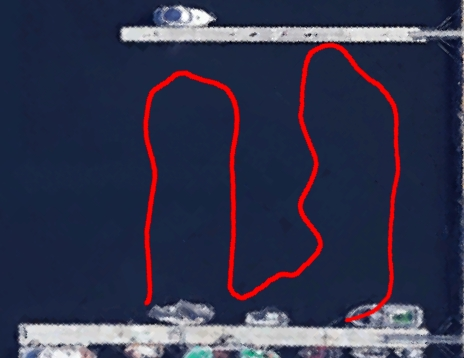
\includegraphics[width=1.0\textwidth]{fig/results/gnss_1.jpg}
		\caption{}
		\label{fig:res2_gnss}
	\end{subfigure}
	\begin{subfigure}[t]{0.5\textwidth}
		\centering
		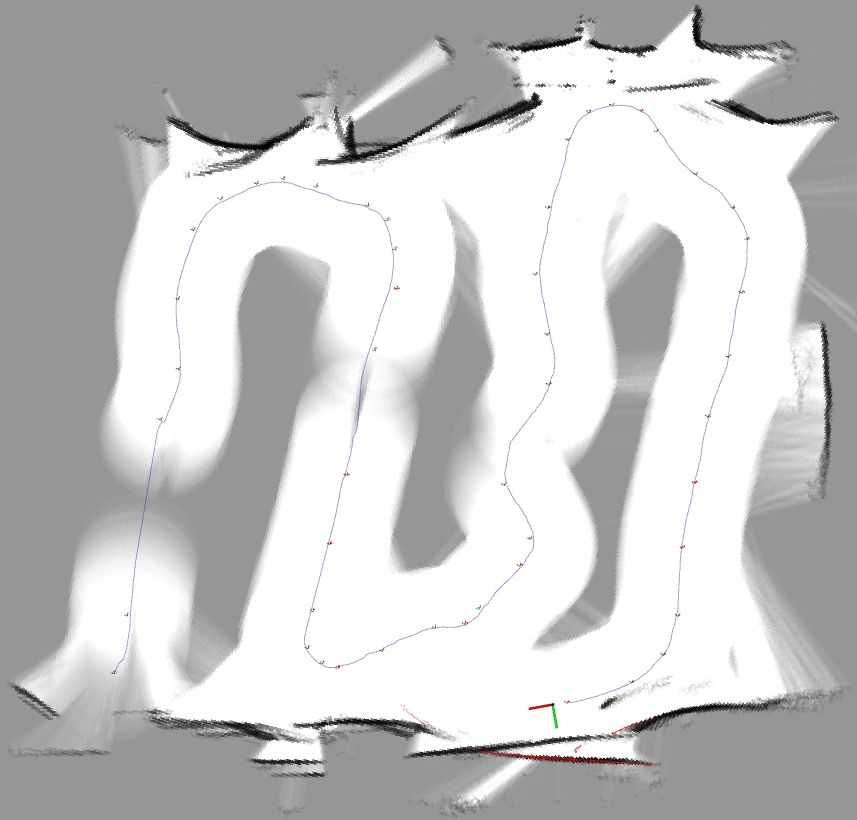
\includegraphics[width=1.0\textwidth]{fig/results/res2_slam_2.jpg}
		\caption{}
		\label{fig:res2_slam}
	\end{subfigure}
	}
	\caption[State at the end of the first experiment.]{State at the end of the first experiment. The starting position was at the left end of the trajectories. (a) GNSS trajectory overlaid an aerial photo. (b) Trajectory and map by SLAM. The white area of the map represents free space, the black area represents obstacles, and the gray area is unknown. Transparent colors mean uncertainty.}
	\label{fig:res2_trajectory}
\end{figure} 

\begin{figure}[h!]
    \centering
    \makebox[\linewidth][c]{
	\begin{subfigure}[b]{0.5\textwidth}
		\centering
		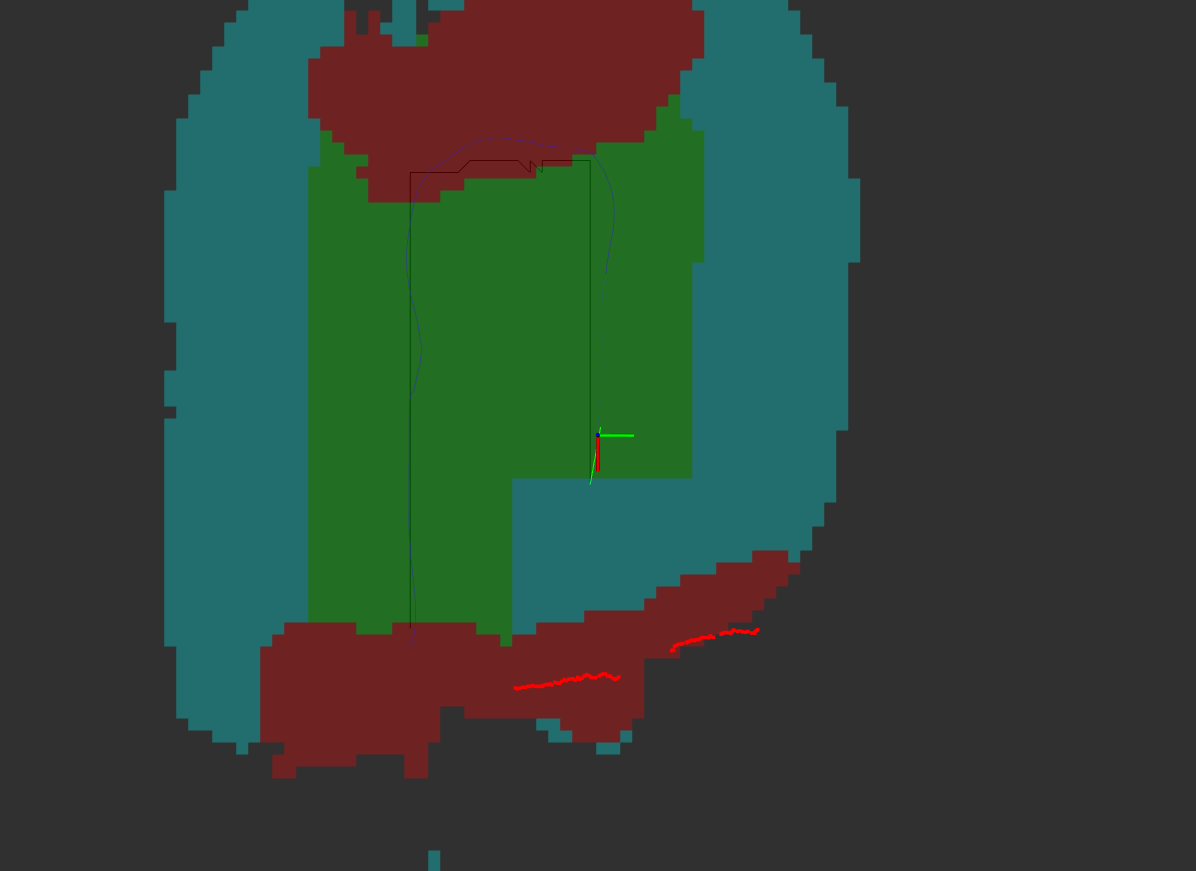
\includegraphics[height=0.25\textheight,width=1\textwidth]{fig/results/ex1_alg1}
		\caption{}
	\end{subfigure}
	\begin{subfigure}[b]{0.5\textwidth}
		\centering
		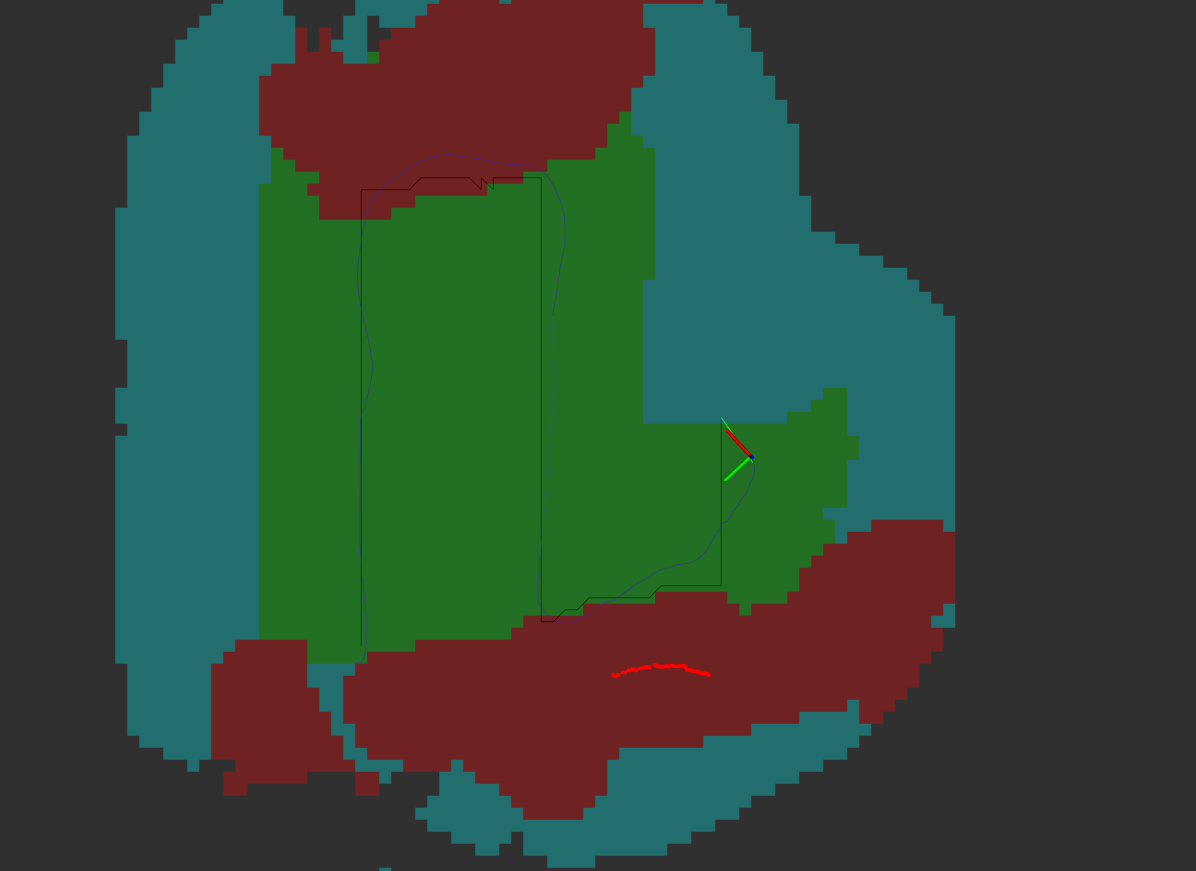
\includegraphics[height=0.25\textheight,width=1\textwidth]{fig/results/ex1_alg2}
		\caption{}
	\end{subfigure}
	}
	\makebox[\linewidth][c]{
	\begin{subfigure}[b]{0.5\textwidth}
		\centering
		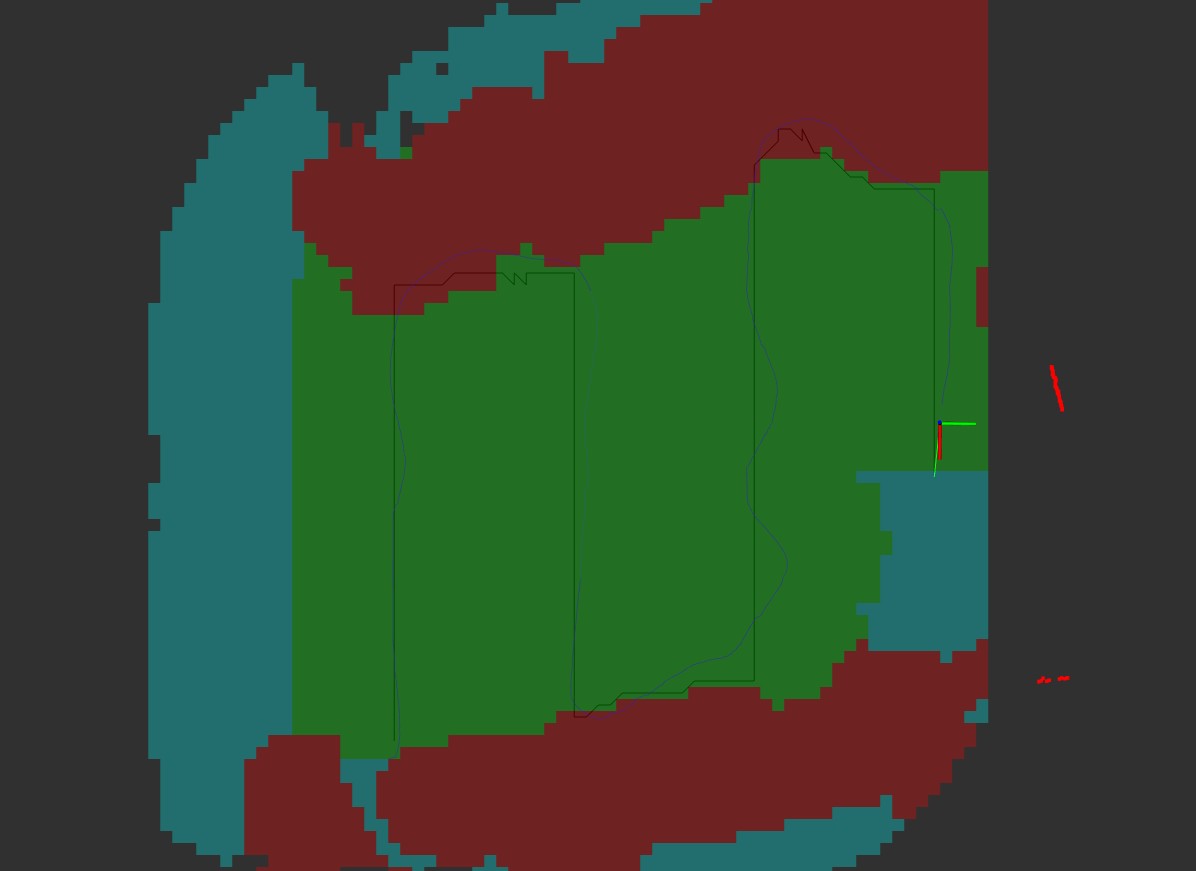
\includegraphics[height=0.25\textheight,width=1\textwidth]{fig/results/ex1_alg3}
		\caption{}
	\end{subfigure}
	\begin{subfigure}[b]{0.5\textwidth}
		\centering
		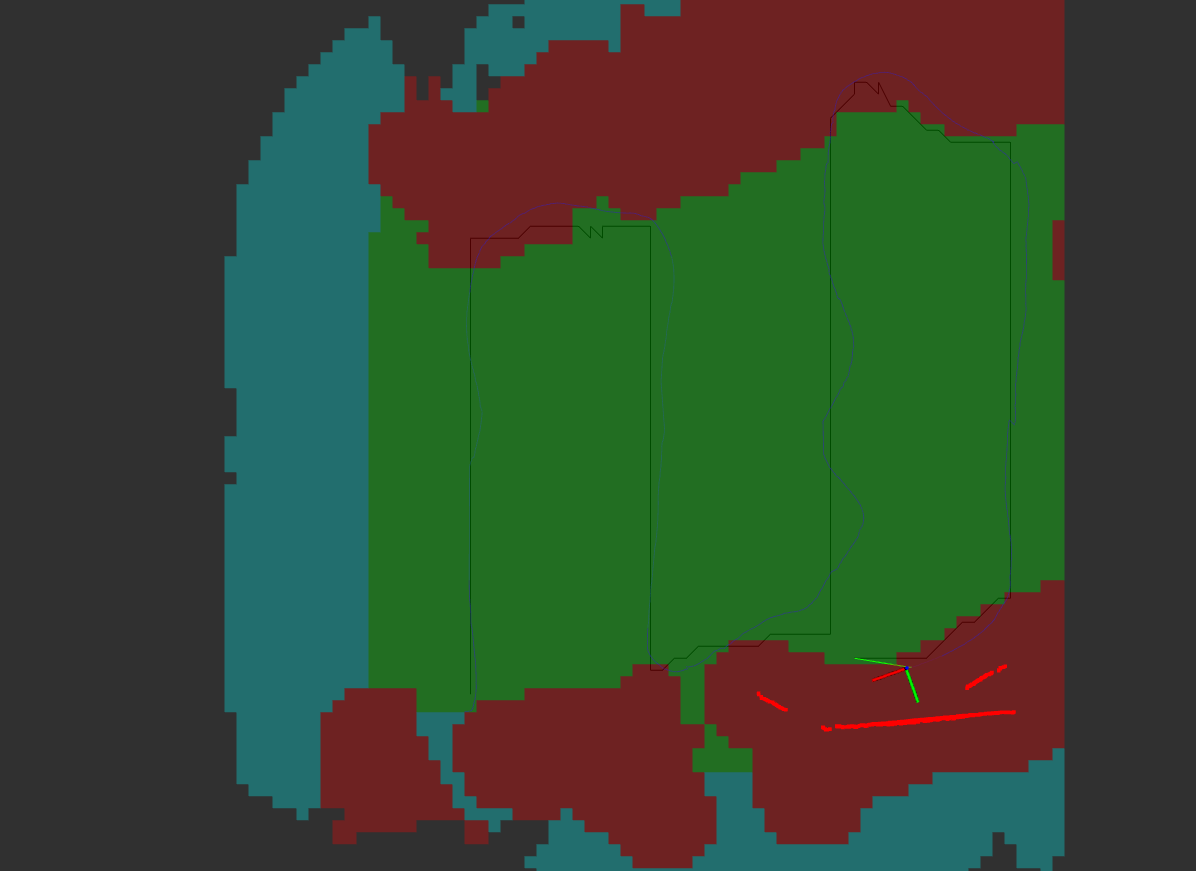
\includegraphics[height=0.25\textheight,width=1\textwidth]{fig/results/ex1_alg4}
		\caption{}
	\end{subfigure}
	}
\caption[Visualization of the boustrophedon motions method at several stages during the first experiment]{Visualization of the boustrophedon motions method at several stages during the first experiment. The red-green-blue axis is the pose of the USV (z-axis positive upwards). Free covered area is green, free uncovered area is blue, and inflated obstacles are red. The light-red dots are current lidar detections. The black line is the connected waypoints. The blue curve is the estimated trajectory.}
	\label{fig:res2}
\end{figure}

\FloatBarrier

\subsection{Second experiment}

The second experiment consisted of the same setup as in the first experiment with the same system parameters. The resulting trajectory according to the GNSS receiver is shown in \figref{fig:gnss_test2}. \figref{fig:ex2_slam} shows the SLAM map and estimated trajectory at different stages during the experiment. \figref{fig:ex2_res} shows the visualization by the system during different stages of the experiment. The USV reaches the right edge of the target region in \figref{fig:ex2_res}b, which is why the visualization does not expand further right. The experiment was aborted at the end because the system's estimated position deviated too much from the observed position.

\newgeometry{top=2.5cm,right=1.7in,left=1.7in,bottom=2.5cm}

\begin{figure}[h!]
	\centering
	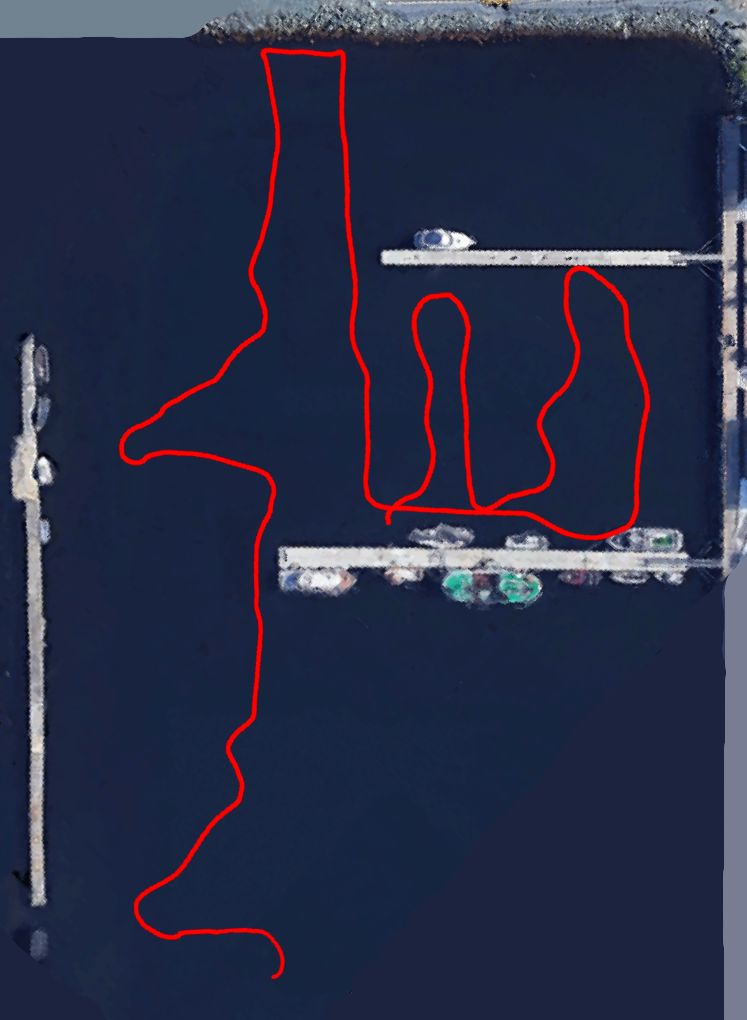
\includegraphics[height=0.3\textheight]{fig/results/gnss_3.jpg}
	\caption{GNSS trajectory in the second experiment.}
	\label{fig:gnss_test2}
\end{figure}

\begin{figure}[h!]
    \centering
    \makebox[\linewidth][c]{
	\begin{subfigure}[b]{0.5\textwidth}
		\centering
		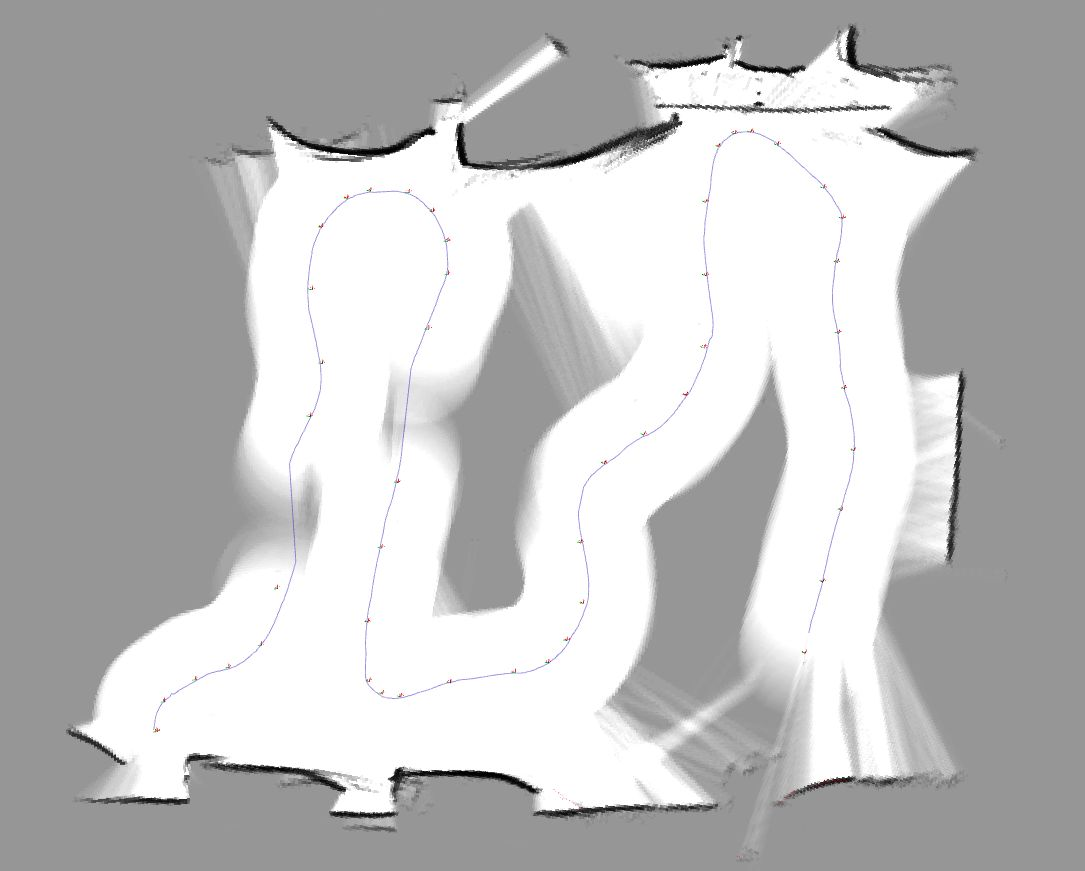
\includegraphics[width=1\textwidth]{fig/results/ex2_slam_1}
		\caption{}
	\end{subfigure}
	\begin{subfigure}[b]{0.5\textwidth}
		\centering
		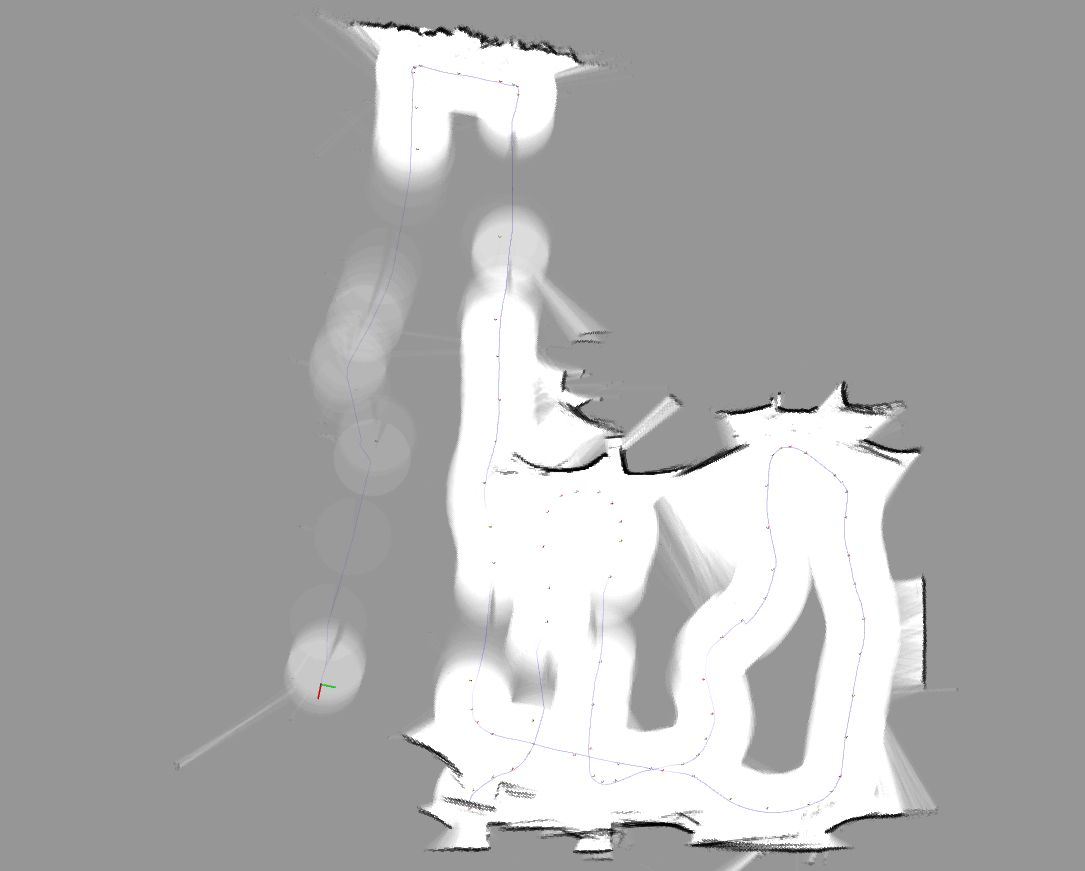
\includegraphics[width=1\textwidth]{fig/results/ex2_slam_2}
		\caption{}
	\end{subfigure}
	}
	\makebox[\linewidth][c]{
	\begin{subfigure}[b]{0.5\textwidth}
		\centering
		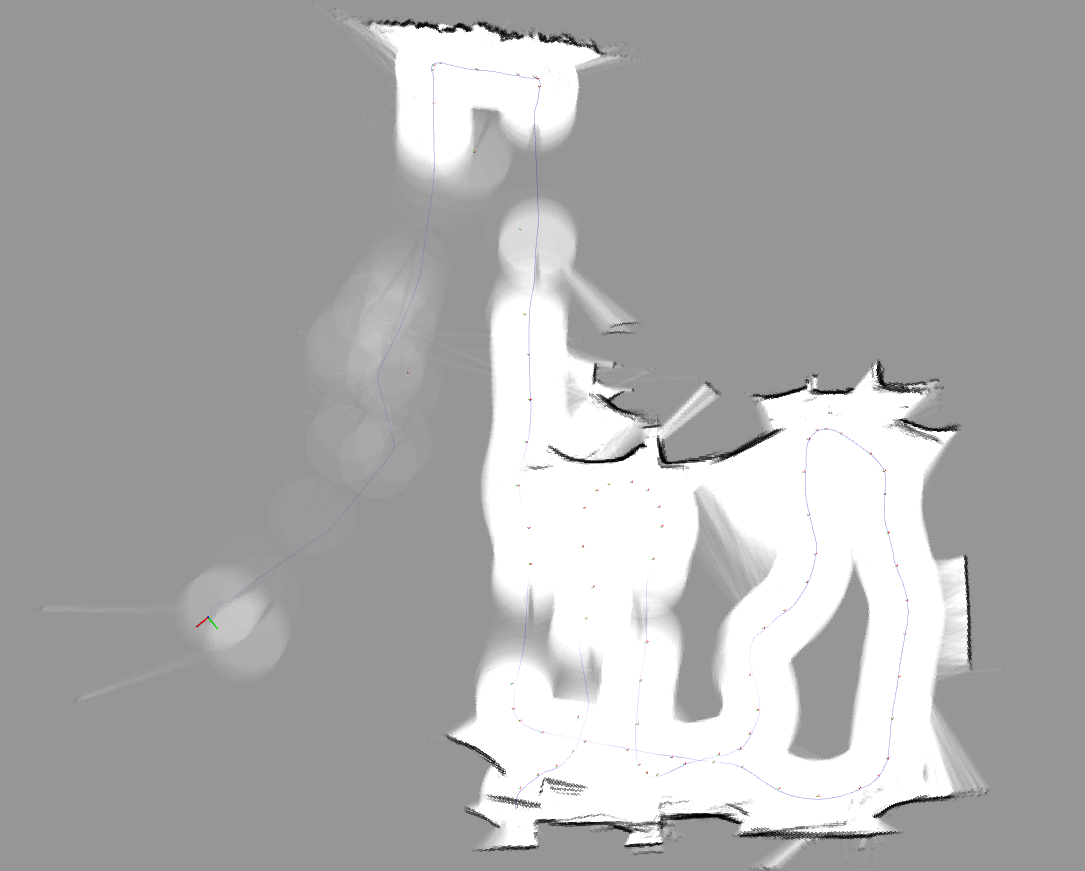
\includegraphics[width=1\textwidth]{fig/results/ex2_slam_nice}
		\caption{}
	\end{subfigure}
	\begin{subfigure}[b]{0.5\textwidth}
		\centering
		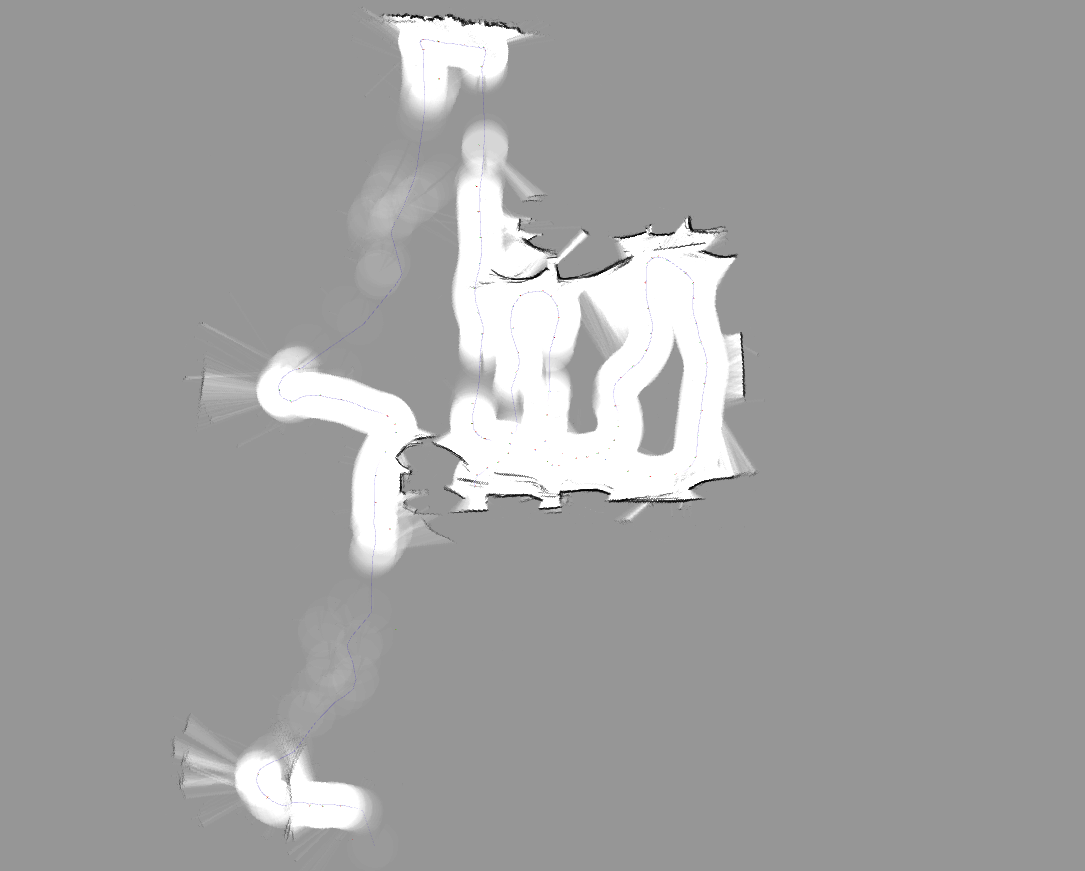
\includegraphics[width=1\textwidth]{fig/results/ex2_slam_nice2}
		\caption{}
	\end{subfigure}
	}
\caption[Trajectory and map according to the SLAM system Cartographer at different stages of the second experiment.]{Trajectory and map according to the SLAM system Cartographer at different stages of the second experiment. The white area of the map represents free space, the black area represents obstacles, and the gray area is unknown. Transparent colors mean uncertainty.}
	\label{fig:ex2_slam}
\end{figure}

\begin{figure}[h!]
    \centering
    \makebox[\linewidth][c]{
	\begin{subfigure}[b]{0.5\textwidth}
		\centering
		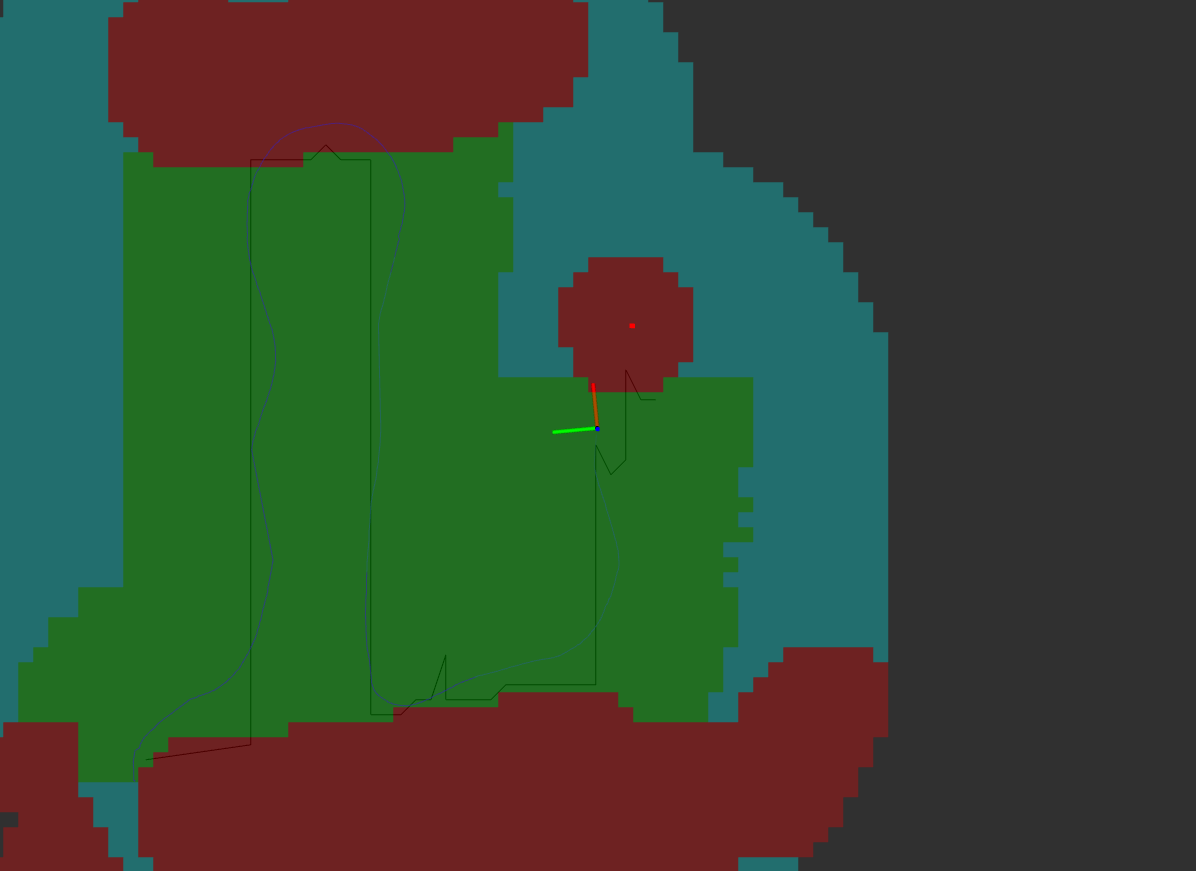
\includegraphics[height=0.25\textheight,width=1\textwidth]{fig/results/ex2_alg3}
		\caption{}
	\end{subfigure}
	\begin{subfigure}[b]{0.5\textwidth}
		\centering
		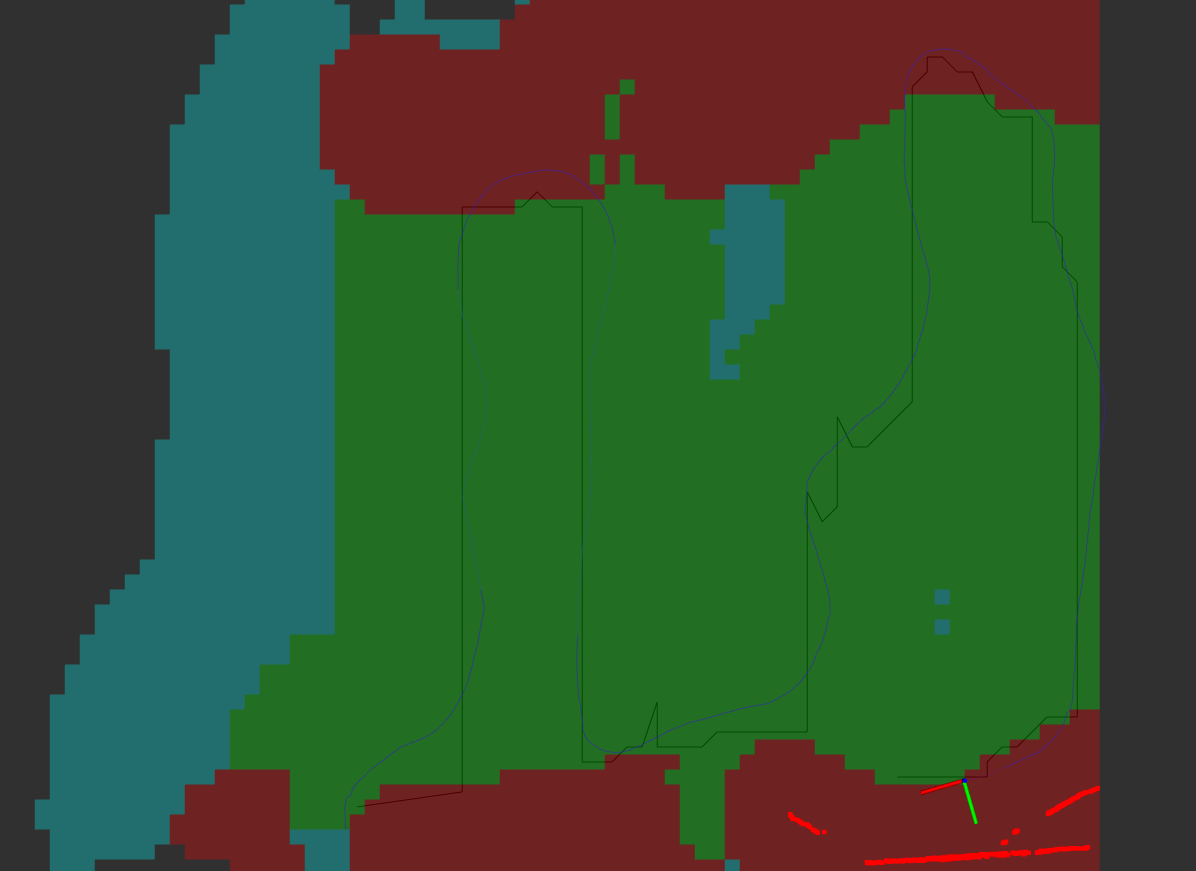
\includegraphics[height=0.25\textheight,width=1\textwidth]{fig/results/ex2_alg7}
		\caption{}
	\end{subfigure}
	}
		\makebox[\linewidth][c]{
	\begin{subfigure}[b]{0.5\textwidth}
		\centering
		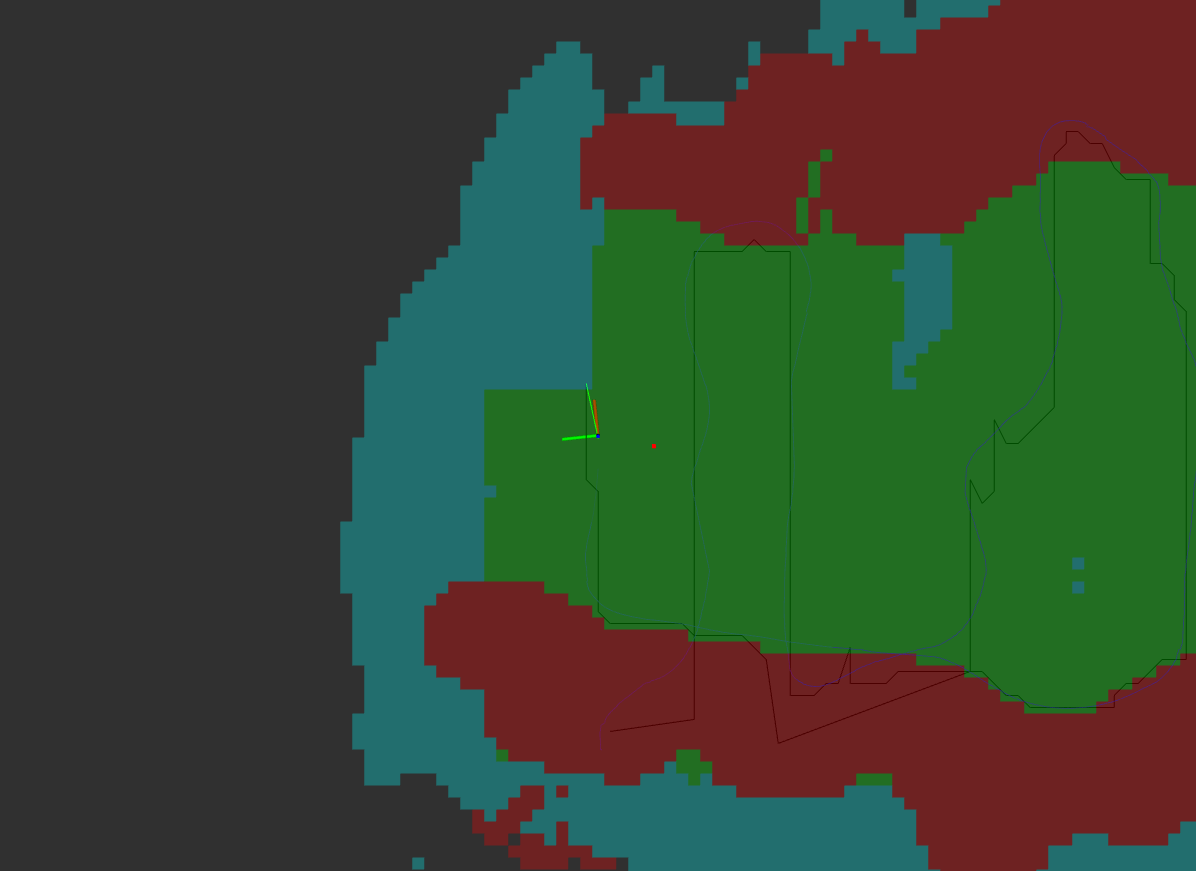
\includegraphics[height=0.25\textheight,width=1\textwidth]{fig/results/ex2_alg_1}
		\caption{}
	\end{subfigure}
	\begin{subfigure}[b]{0.5\textwidth}
		\centering
		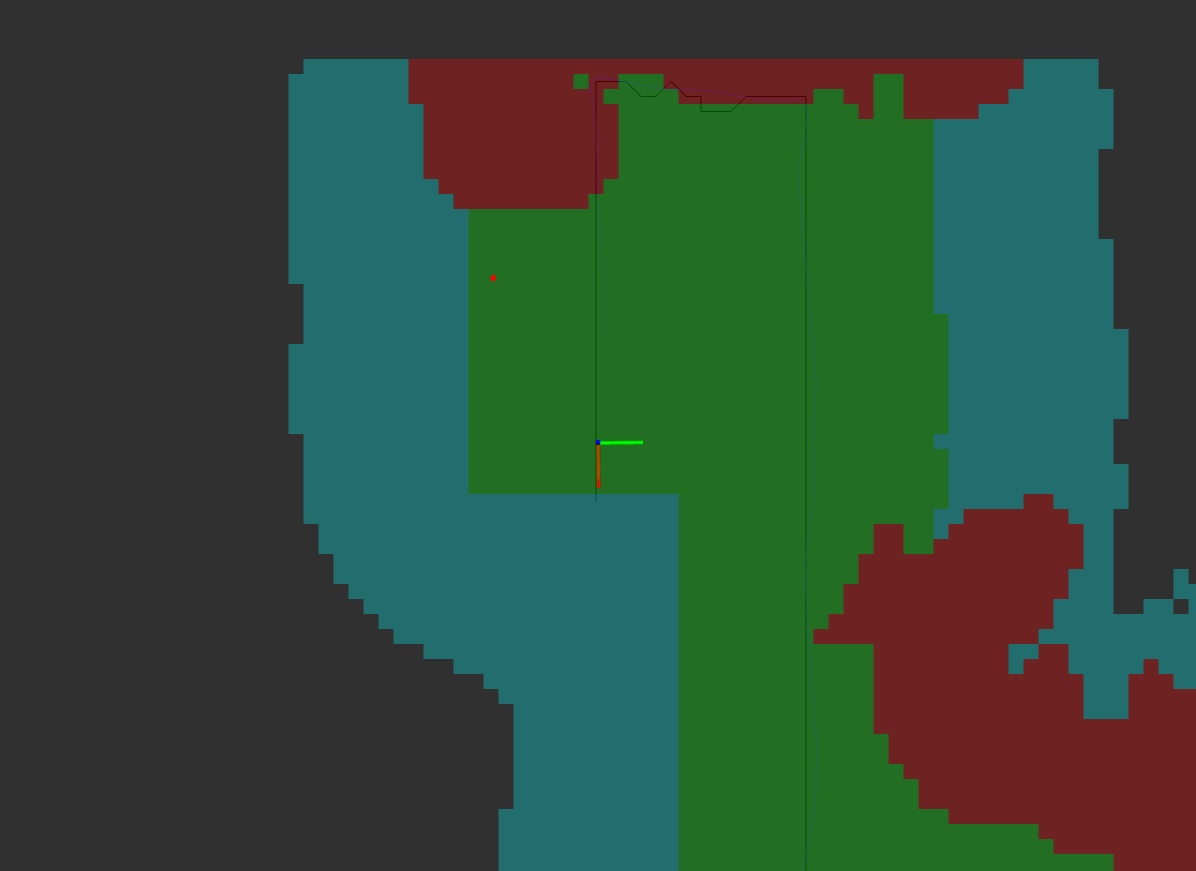
\includegraphics[height=0.25\textheight,width=1\textwidth]{fig/results/ex2_alg9}
		\caption{}
	\end{subfigure}
	}
	\makebox[\linewidth][c]{
	\begin{subfigure}[b]{0.5\textwidth}
		\centering
		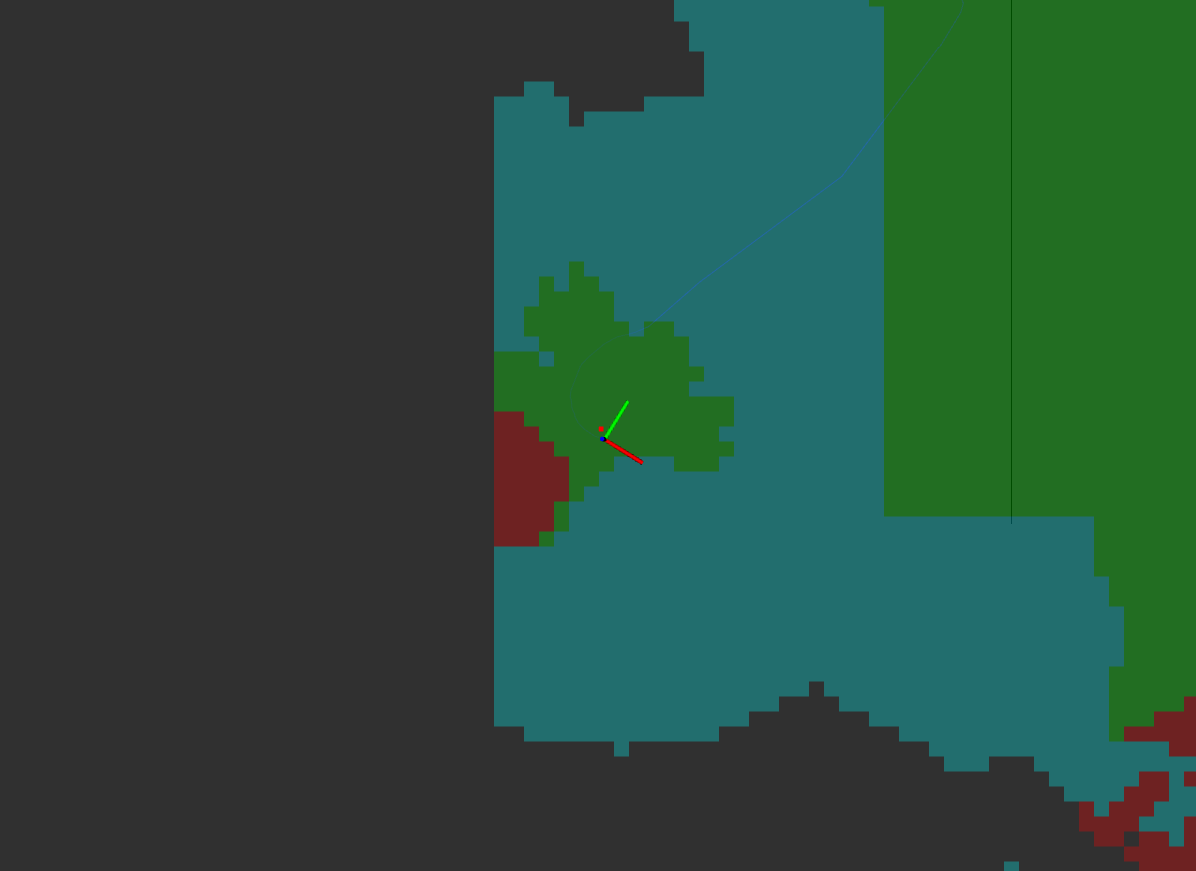
\includegraphics[height=0.25\textheight,width=1\textwidth]{fig/results/ex2_alg11}
		\caption{}
	\end{subfigure}
	\begin{subfigure}[b]{0.5\textwidth}
		\centering
		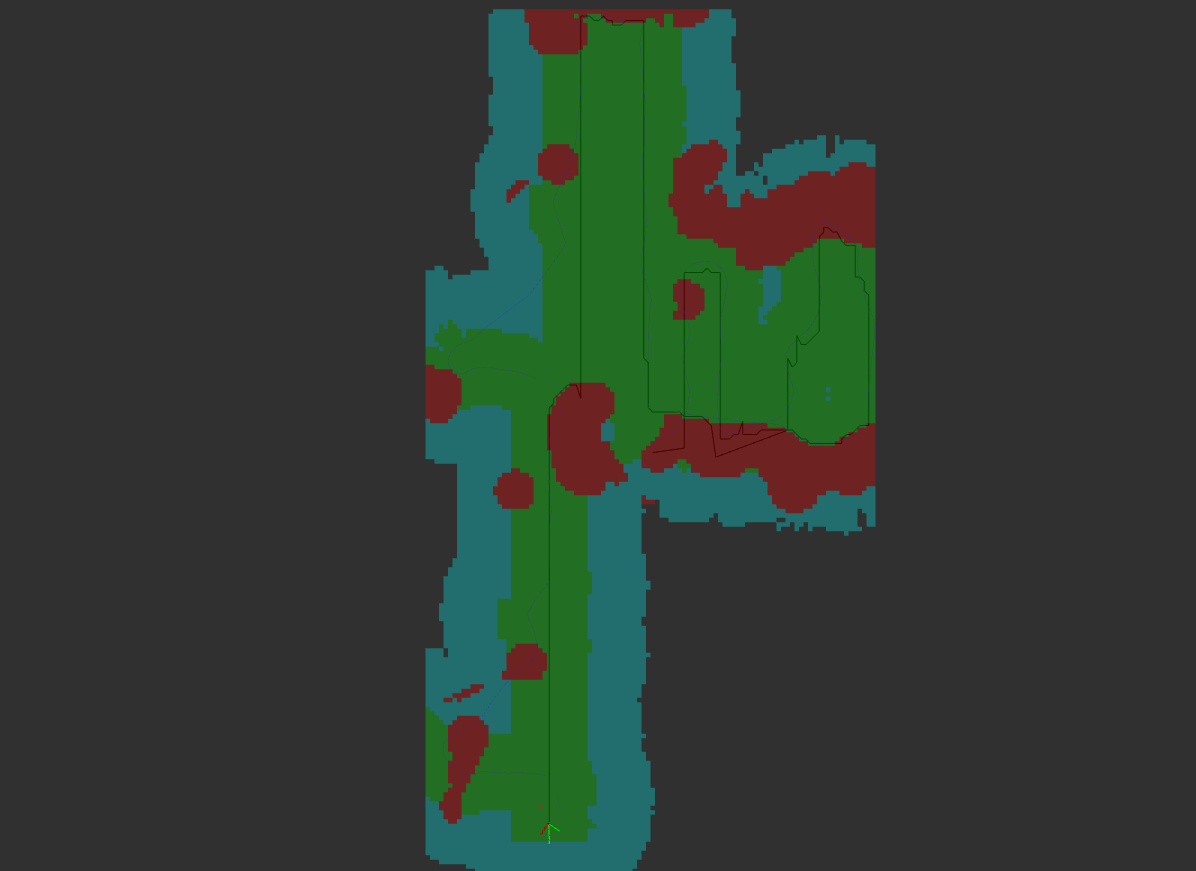
\includegraphics[height=0.25\textheight,width=1\textwidth]{fig/results/ex2_alg_2}
		\caption{}
	\end{subfigure}
	}
\caption[Visualization of the boustrophedon motions method at several stages during the second experiment]{Visualization of the boustrophedon motions method at several stages during the second experiment. The red-green-blue axis is the pose of the USV (z-axis positive upwards). Free covered area is green, free uncovered area is blue, and inflated obstacles are red. The light-red dots are current lidar detections. The black line is the connected waypoints. The blue curve is the estimated trajectory.}
	\label{fig:ex2_res}
\end{figure}

\restoregeometry

\FloatBarrier

\section{Discussion}

\subsection{Sensor fusion and SLAM}

\figref{fig:res2_slam} shows the map and trajectory estimated by SLAM for the first experiment. Comparing it to the aerial photo and the GNSS trajectory in \figref{fig:res2_gnss}, there are several signs of drift and deviation in the map. Boats at the top and bottom of the map are not really recognizable as boats, and the jetty at the bottom is drawn twice with a different angle and position. The cause for this is that the SLAM system struggles to accurately localize itself, and so multiple things are mapped on top of each other, resulting in the cluttered map seen in the figure. The top and bottom jetties are also shifted a little sideways compared to each other, so the paths that appear perpendicular to the jetties in the aerial photo, appear sloped in the SLAM map.

 On the other hand, the SLAM trajectory seems to approximate the GNSS trajectory very well, which might mean that there are some inconsistencies in the transformations between the lidar and IMU. However, that does not explain what happens to the mapping of the boats in the top left corner of the SLAM map. Those errors are more likely caused by a drift in the orientation. In fact, during the experiment when the USV moved straight forward, the estimated position was seen to move at an angle compared to the heading (this can be seen at some times in the attached video). This strongly suggest a consistent offset between the estimated orientation and the real orientation. Keep in mind that the GNSS trajectory does not necessarily depict the actual ground truth (it has the standard GNSS accuracy), but it is the closest thing available and will therefore be treated as a ground truth in the discussion.

%Exactly why the SLAM system struggled is hard to pinpoint, but several factors were observed during the experiments.
There are also other factors that were observed to affect the SLAM system during the experiment. The mounted lidar states a range of $\SI{25}{\meter}$, which will be somewhat reduced in outdoor operation. However, in the experiments, the lidar never detected anything more than about $\SI{14}{\meter}$ away. Furthermore, this was only when the lidar rays hit the obstacle's surface at a right angle. When the lidar rays hit the surface with an angle, the range was observed to drop much lower. Dark objects, because of their low reflectivity, were the most difficult to detect. Some objects, like ships with a black hull, were not detected at all. The single scan plane of the lidar also caused some trouble. The lidar was mounted relatively high on the USV, so the jetty at the top of the SLAM map was too low to be seen when the USV moved towards the jetty. Luckily, there was a detectable boat on the other side of the too low jetty that prevented the USV from crashing. Because the USV has a small pitch angle when moving forward, the jetty was seen when moving away and appears in the SLAM map. 

In the second experiment, the mapping of the same area is better, as seen in \figref{fig:ex2_slam}a. The top and bottom jetty is still shifted a little sideways compared to each other, causing the almost perpendicular laps of \figref{fig:gnss_test2} to appear slightly sloped in the SLAM map. In \figref{fig:ex2_slam}b, the SLAM system failed to recognize the bottom jetty when backtracking to the left, which once again seems to have been caused by a drift in orientation. No system parameters were changed between the two experiments, so it is a bit unclear as to why this SLAM map is better. The weather did change though, becoming a little sunnier. This caused a lot of false detections in the lidar, which is not clear from the SLAM map because only persistent detections appear in the map. However, the instantaneous data from the lidar used in the rolling window was affected. This had an impact on path planning which is discussed in the next section.

In \figref{fig:ex2_slam}b the SLAM system has gone a long time without any lidar detections, and the map becomes very uncertain because of it (transparent white in the figure). The lack of lidar detections means the SLAM system must depend entirely on GNSS and IMU for localization. This should cause no trouble if the fusing of GNSS and IMU data is good. However, the current pose and recent trajectory of the USV in \figref{fig:ex2_slam}b deviates a lot from the GNSS trajectory in \figref{fig:gnss_test2}. In \figref{fig:ex2_slam}c, only a couple of seconds later, Cartographer actually realizes this and corrects for it. Note that this means the fused GNSS and IMU data must have been available all the time, but is only incorporated correctly after the lidar starts detecting obstacles again. This most likely means that the implementation of Cartographer runs some of its graph optimizations only after it has received a certain number of lidar detections.
The documentation states that "the optimization is run in batches once a certain number of trajectory nodes was inserted" \citep{website:CartographerRos}. Based on the obtained results, the generation of these trajectory nodes likely requires lidar detections. This makes the proposed setup in Cartographer very poorly suited for open marine environments, especially when using a short range lidar. Exactly the same thing happens once more in the experiment, and can be seen in \figref{fig:ex2_slam}d. After that, the experiment was aborted. The fact that the USV drifts in the same direction both times, further emphasizes the possibility of an error in the orientation estimation.

\subsection{CCPP with boustrophedon motions}

The GNSS trajectory of the first experiment is shown in \figref{fig:res2_gnss}, and it clearly depicts a  boustrophedon motion between the jetties. \figref{fig:res2} shows that the system also manages to achieve complete coverage for this area. Obstacles are identified correctly by the system, and the CCPP method successfully plans a collision-free path that steers clear of them. The planned path can be seen inside the inflated obstacles region at some places, or further into the free space region than it should be. This is because the status of the cells has changed after the USV reached those waypoints. The large inaccuracies in localization and mapping experienced during this test makes this very noticeable.

At the very end of the experiment, just after \figref{fig:res2}d, the system ended up planning a backtracking path straight through the obstacles seen at the bottom. This was caused by an error in the implementation of the system that incorrectly dealt with multiple status changes in a cell, e.g. caused by mapping inaccuracies. This was discovered and fixed before the second experiment. However, it does illustrate the fact that the CCPP method contains very little logic for dealing with uncertainties. Currently, the only logic aimed at this is the fact that the system replans the next waypoint if it becomes blocked.

The results of the second experiment are largely influenced by false lidar detections due to sunlight, and localization drift. The GNSS trajectory in \figref{fig:gnss_test2} shows that the USV first covers the area between the jetties with a single boustrophedon motion. The laps are not as nice and straight as in the previous experiment, but this is because the system avoids the non-existing obstacles reported by false lidar detections. Next, the system backtracks and starts a new boustrophedon motion. This motion suffers from two detours. The cause of the detours was, as explained in the last section, due to localization drift. After the second detour the experiment is aborted.  Even though the resulting trajectory is not as good as in the simulations, it does show the system's main properties working in a real-world environment. Namely, boustrophedon motions and backtracking.

The subfigures of \figref{fig:ex2_res} show a closer look at how the CCPP method reacted during the second experiment. In \figref{fig:ex2_res}a, a false detection appears in front of the USV. Since it is so close to the USV, this false detection causes the USV to wall follow to the side of it. Note that it is not just a single false detection that causes this, but several. They appear, the obstacle is inflated, the path is replanned, and then they disappear. The turn at the very beginning of the boustrophedon motion, in the lower left corner, was not caused by false detections. This was due to the USV's starting position being inside the inflated obstacles region. This is a situation that is not explicitly considered in the implemented system, but since the system planned a path anyway, it is not entirely safe.

For the rest of the subfigures in \figref{fig:ex2_res}: (b) After wall following to the side of the false obstacle in (a) and of another one on the way down, there are two small uncovered regions remaining within the covered area. A possible extension of the system would therefore be to wall follow not just to the side of obstacles, but around them. This would have covered these remaining areas. (c) The USV backtracks and begins another boustrophedon motion to the left of the starting point (the method was slightly altered for this experiment to ignore the closer but very small enclosed uncovered areas). The sweeping direction is switched because of a false detection. (d) Since the sweeping direction was switched, the USV now continues back down on the left. (e) The jump in the position of the SLAM system moves the USV far out from the desired path. (f) The USV manages to get back on the path after the jump in position. A new jump appears, and the same thing happens. When the localization drifts as much as it did in this experiment, the coverage reported by the system is not correct anymore. After loop closures and trajectory adjustments, the coverage should ideally be recalculated based on the new estimated trajectory. In this experiment, however, even the trajectory with loop closure at the end had significant uncorrected drift which would later have caused problems.

\subsection{Path following}

The localization in both experiments is not really sufficient for making accurate conclusions about the performance of the path following method. The estimated trajectory is adjusted several times during the experiment by the SLAM system, while the planned path is kept still throughout the whole experiment. Furthermore, it should be kept in mind that the planned path in all figures are the waypoints connected by line segments, and not the actual simple Dubins paths followed.

Even with the poor localization, the USV still managed to track the paths. In \figref{fig:res2}, the estimated trajectory seems to follow the planned path reasonably well most of the time. The same is true for \figref{fig:ex2_res}. The path following method has therefore been proved to be robust, and should be considered satisfactorily in both experiments. There are significant deviations several places, but it is hard to tell whether they are because of the path following, localization, or both. However, the path following is definitely to blame for some of it. In the first experiment, there are some oscillations in the third lap, see \figref{fig:res2}c. This may seem to be because of bad path following, but it is clear from looking at logged data of the experiment that these oscillations are largely affected by pose adjustments of the SLAM system (it can also be seen from the attached video).

All these problems with localization also made it very hard to tune the parameters of the system. A significant performance increase in path following is therefore likely achievable by better tuning of the system. One thing that managed to make the system very reliable and safe during the experiments, was the buffer safety zone that is added around all obstacles. This allowed for many smaller things to go wrong, while still making sure the complete system functioned as a whole and avoided collisions.

